
%==============================================================================
\section{Model description} \label{sec_model}
%==============================================================================

\subsection{Agents and rules}

The world is represented by a square lattice $(L_{i,j})_{1\leq i,j\leq N}$ composed of cells that are empty or occupied (Fig.~\ref{fig_lattice}). This is denoted by a function $\delta(i,j,t)\in\{0,1\}$, where time $t$ follows an iterative sequence $t\in\mathbb{T} = \tau\mathbb{N} = \{0, \tau, 2\tau, ...\}$~\cite{golden2012modeling} with a regular time step $\tau$. Another evolving structure is laid out on top of the lattice: a Euclidean network $G(t)=(V(t),E(t))$ whose vertices $V$ are a finite subset of the world and edges $E$ (its agents) represent \emph{roads}. In the beginning, the lattice is empty: $\delta(i,j,0)=0$, and the network is either initialized randomly (e.g.~uniformly) or set to a user-specified configuration $G(0)=(V_0,E_0)$. In order to translate functional mechanisms into the growth of a city, we assume that the initial vertices include a subset formed by \emph{city centers}, $C_0\subset V_0$, which have integer \emph{activities}, denoted by $a:C_0\rightarrow\{1,\ldots,a_{\max}\}$.

To characterize the urban structures emerging in this world, we define in general a set of $k$ functions of the lattice, $(d_k(i,j,t))_{1\leq k\leq K}$, called \emph{explicative variables}. These variables are here: $d_1$, the \emph{density}, i.e.~the average $\delta$ around a cell $(i,j)$ in a circular neighborhood of radius $\rho$; $d_2$, the Euclidean \emph{distance} of a cell to the nearest road; $d_3$ the \emph{network-distance} of a cell to the nearest city center, i.e.~the sum of $d_2$ and edge lengths; and $d_4$, the \emph{accessibility} of activities (or rather difficulty thereof), written
%
\begin{equation}
d_4(i,j,t)=\left(\frac{1}{a_{\max}}\sum_{a=1}^{a_{\max}}d_3(i,j,t;a)^{p_4}\right)^{1/p_4}
\end{equation}
%
where $d_3(i,j,t;a)$ is the network-distance of the cell to the nearest center with an activity $a$, and $p_4\geq1$ (typically~3) defines a $p$-norm.

A set of weights $(\alpha_k)_{1\leq k\leq K}\in[0,1]^K$ is assigned to these variables to tune their respective influence on what we define as the net \emph{land value} of a cell, as follows:
%
\begin{equation}
v(i,j,t)=\frac{1}{\sum_k \alpha_k}\sum_{k=1}^K \alpha_k\;\frac{d_{k,\max}(t)-d_k(i,j,t)}{d_{k,\max}(t)-d_{k,\min}(t)}.
\end{equation}

\noindent Houses are preferentially built where $v$ is high, i.e.~$d_k$'s are low. Thus the evolution of the system proceeds in three phases at each time step: (a)~all values $v(i,j)$ are updated, (b)~among the cells that have the best values, $n$ new cells are randomly chosen and ``built'' (set to $\delta=1$); (c)~for each built cell, if $d_2$ is greater than a threshold $\theta_2$ (maximum isolation distance), then that cell is directly connected to the network by creating a new road branching out orthogonally from the nearest edge.

Network initialization is random (see details in~\ref{sec_extval}), and the selection of new cells is also random among identical values of~$v$. A sensitivity analysis and model exploration is conducted in the next section to determine the relative effect of parameters with respect to these sources of randomness. In any case, growth is halted after a constant amount of time $T$, evaluated from experiments, so that the final structure is neither ``unfinished'' nor filling out the world (see~\ref{sec_extval}). Fig.~\ref{fig_flowchart} displays the core ABMS flowchart with feedback interactions between agents.

\begin{figure}[t]
\centering
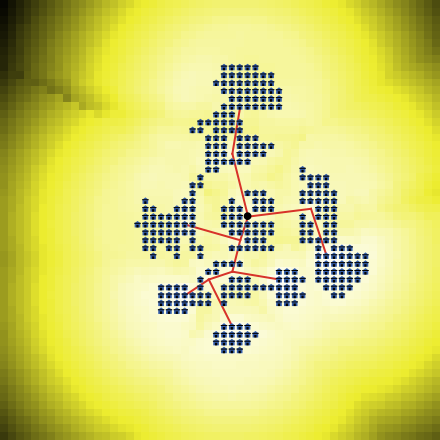
\includegraphics[width=0.9\columnwidth]{figures/lattice}
\caption{\small Example of urban morphology generated by the model. Houses (blue squares) were built in some cells of a $56\times 56$ lattice. City centers and roads (red edges) compose the added network. Cell shades (yellow) represent distances to the built cells (the brighter, the closer).}
\label{fig_lattice}
\vspace{0.5cm}
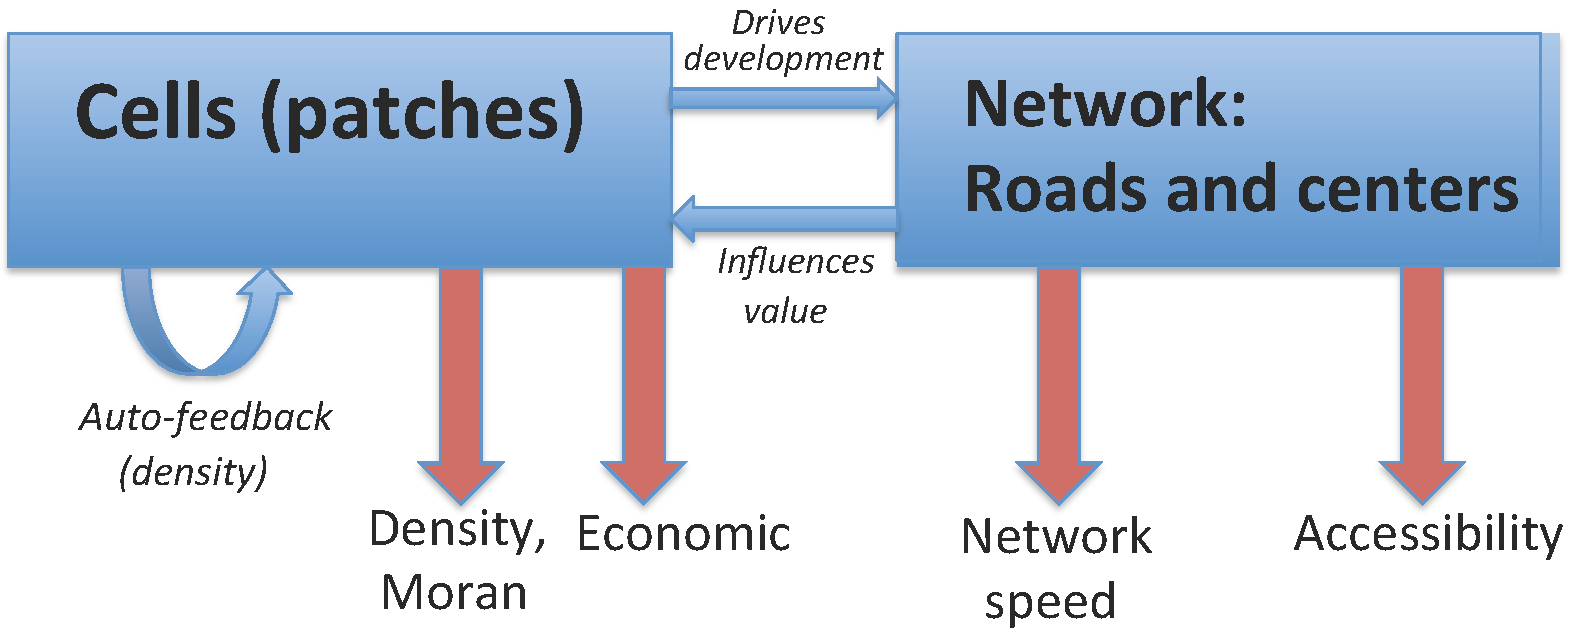
\includegraphics[width=0.9\columnwidth]{figures/flowchart}
\caption{\small The hybrid network/grid model. \emph{Blue arrows}: feedback interactions. \emph{Red arrows}: output evaluation functions.}
\label{fig_flowchart}
\end{figure}

\subsection{Evaluation functions}

Once a structure is generated, its properties need to be quantified so that it can be categorized or compared to other structures for optimization purposes. To this goal, we define various \emph{evaluation functions}, both objective quantification measures and structural fitness values. The measures described in this section take into account all the explicative variables, whose distributions over the grid are emergent properties that cannot be known in advance and are therefore essential to monitor.

\paragraph{Morphology}

To assess the morphological structure of an urban configuration, we map it onto a 2D metric space defined by a pair of global indicators $(D,I)$ called the \emph{integrated density} and the \emph{Moran index} (Fig.~\ref{fig_morpho}). The density $D\in[0,1]$ is calculated by taking the $p$-norm (with exponent $p_D\geq 1$, typically 3) of the local densities $d_1$:
\begin{equation}
D(t)=\left(\frac{1}{\sum_{i,j} \delta(i,j,t)}\!\!\sum_{\scriptstyle i,j=1\atop\scriptstyle\delta(i,j,t)\neq0}^N\!\!d_1(i,j,t)^{p_D}\right)^{1/p_D}
\end{equation}
%
\noindent Moran's $I$, an index of spatial autocorrelation, is widely used in quantitative geography~\cite{tsai2005quantifying,lenechet:hal-00696445} to evaluate the ``polycentric'' character of a distribution of populated cells. It is defined by
%
\begin{equation}
I(t)=\frac{M^2}{\sum_{\mu\neq\nu} 1/d_{\mu\nu}}\frac{\sum_{\mu\neq\nu} (P_\mu-\overline{P})(P_\nu-\overline{P})/d_{\mu\nu}}{\sum_{\mu=1}^{M^2}(P_\mu-\overline{P})^2}
\end{equation}
%
where the lattice is partitioned into $M\times M$ square areas, at an intermediate scale between cell size and world size ($1\ll\!M\ll\!N$), $d_{\mu\nu}$ is the distance between the centroids of areas $\mu$ and $\nu$, $(P_\mu)_{1\leq\mu\leq M^2}$ denotes the number of occupied cells in each area, and $\overline{P}$ is their global average. We can recognize in this formula the normalized ratio of a modified covariance (pairwise correlations divided by distances) and the variance of the distribution. Moran's $I$ belongs by construction to the interval $[-1,1]$, where values near 1 correspond to a strong monocentric distribution, values around 0 to a random distribution, and values near $-1$ to a checkered pattern (every other cell occupied). Usually, polycentric distributions have relatively small positive $I$ values, depending on the size and distance between centers.

\paragraph{Network performance}

Due to the branching nature of the growth algorithm, the network of roads $G$ cannot contain any other loops than the ones initially present in $G_0$. Therefore, notions of ``clustering coefficient'' or ``robustness'' (with respect to node removal) are not relevant here. On the other hand, since $G$ is intended to simulate a \emph{mobility} network, we can evaluate its performance by defining a \emph{relative speed}~\cite{banos2012towards} $S$, representing the ``detours'' imposed by $G$ with respect to direct, straight travels:
%
\begin{equation}
S(t)=\left(\frac{1}{\sum_{i,j}\delta(i,j,t)}\!\!\sum_{\scriptstyle i,j=1\atop\scriptstyle\delta(i,j,t)\neq0}^N\!\!\left(\frac{d_3(i,j,t)}{e_3(i,j,t)}\right)^{p_S}\right)^{1/p_S}
\end{equation}
%
\noindent where $p_S\geq 1$ (also 3), and $e_3(i,j,t)$ is the direct Euclidean distance between cell $(i,j)$ and the nearest city center over the network, i.e.~the one that realizes the value of $d_3(i,j,t)$. Note that $S\ge1$ and is actually higher for more convoluted networks (thus it is a measure of ``slowness'', but we still employ ``speed'').

\paragraph{Functional accessibility}

The global functional accessibility $A$ to city centers is another $p$-norm (also 3), based on the relative local accessibility from each cell, which is $d_4$ over its maximum:
%
\begin{equation}
A(t)=\left(\frac{1}{\sum_{i,j}\delta(i,j,t)}\!\!\sum_{\scriptstyle i,j=1\atop\scriptstyle\delta(i,j,t)\neq0}^N\!\!\left(\frac{d_4(i,j,t)}{d_{4,\max}(t)}\right)^{p_A}\right)^{1/p_A}
\end{equation}

\noindent This normalization puts $A$ in $[0,1]$ and allows comparing configurations of different sizes. Like $S$, ``better'' urban configurations are characterized by a lower $A$.

\paragraph{Economic performance}

It was shown by Banos~\cite{banos2012network} that the Schelling segregation model, a standard ABM of socio-economic dynamics~\cite{schelling1969models}, was highly sensitive to the spatial structures in which it could be embedded, since segregation rules depended on proximity. This justifies the use of this model as an evaluation of \emph{economic performance} of our urban configurations, measuring how much structure influences segregation. To this aim, we implemented a model of residential dynamics based on the work of Benenson et al.~\cite{benenson1998multi}. The output function is a segregation index $H(t)$ calculated on the residential patterns that emerge inside a distribution of built patches. For urban structures produced in a practical case (Section~\ref{sec_practapp}), we obtained densities of mobile agents between 0.1 and 0.2. Following Gauvin et al.~\cite{gauvin2009phase}, the phase diagram of the Schelling model indicates that in such a density range, tolerance thresholds of 0.4 to 0.8 lead to clustered frozen states, where the calculation of a spatial segregation index is indeed relevant. The detailed description of this economic model is out of the scope of this paper.




